
\documentclass[tikz,border=2mm]{standalone}

\usepackage{bm}
\usepackage{xcolor}
\usetikzlibrary{arrows,positioning}
\usetikzlibrary{arrows.meta}

\newcommand{\VE}{\ensuremath{\textrm{VE}}}

\definecolor{colorS}{HTML}{56B4E9}
\definecolor{colorRu}{HTML}{009E73}
\definecolor{colorV}{HTML}{F0E442}
\definecolor{colorRv}{HTML}{D55E00}
\definecolor{colorIu}{HTML}{0072B2}
\definecolor{colorIv}{HTML}{E69F00}

\begin{document}

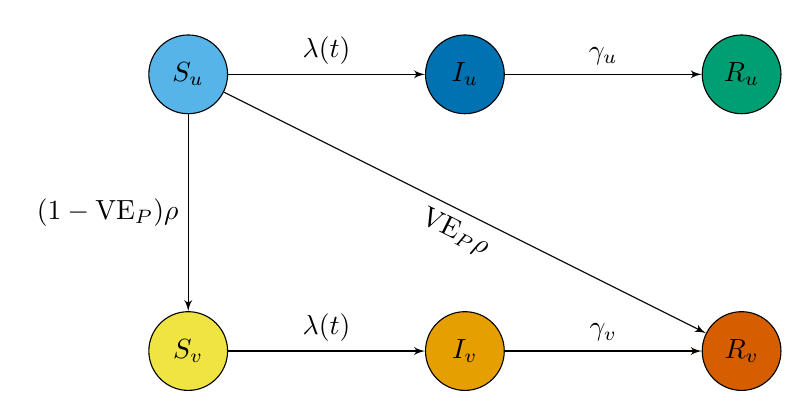
\begin{tikzpicture}[node distance=2.5cm,auto,>=latex',every node/.append style={align=center},int/.style={draw, minimum size=1cm, circle},inverter/.style={rectangle,draw,inner sep=2pt,minimum size=6mm},]
    \node [int, fill=colorV, fill opacity=1, text opacity=1] (V4)             {$S_v$};
    \node [int, above=of V4, fill=colorS, fill opacity=1, text opacity=1] (S4)             {$S_u$};
    \node [int, right=of S4, fill=colorIu] (Is4)             {$I_u$};
    \node [int, right=of Is4, fill=colorRu, fill opacity=1, text opacity=1] (Rs4)             {$R_u$};
    \path[->] (S4) edge node [above] {$\lambda(t)$} (Is4);
    \path[->] (Is4) edge node [above] {$\gamma_u$} (Rs4);
    \node [int, right=of V4, fill=colorIv] (Iv4)             {$I_v$};
    \node [int, right=of Iv4, fill=colorRv, fill opacity=1, text opacity=1] (Rv4)             {$R_v$};
    \path[->] (S4) edge node [left] {$(1-\VE_P) \rho$} (V4);
    \path[->] (S4) edge node [sloped, below] {$\VE_P \rho$} (Rv4);
    \path[->] (V4) edge node [above] {$\lambda(t)$} (Iv4);
    \path[->] (Iv4) edge node [above] {$\gamma_v$} (Rv4);
\end{tikzpicture}
\end{document}

